
\documentclass{beamer}[10pt]
\usepackage{verbatim}
\mode<presentation> {
	
	%\usetheme{default}
	%\usetheme{AnnArbor}
	%\usetheme{Antibes}
	%\usetheme{Bergen}
	%\usetheme{Berkeley}
	%\usetheme{Berlin}
	%\usetheme{Boadilla}
	%%\usetheme{CambridgeUS}
	%\usetheme{Copenhagen}
	%\usetheme{Darmstadt}
	%\usetheme{Dresden}
	%\usetheme{Frankfurt}
	%\usetheme{Goettingen}
	%\usetheme{Hannover}
	%\usetheme{Ilmenau}
	%\usetheme{JuanLesPins}
	%\usetheme{Luebeck}
	\usetheme{Madrid}
	%\usetheme{Malmoe}
	%\usetheme{Marburg}
	%\usetheme{Montpellier}
	%\usetheme{PaloAlto}
	%\usetheme{Pittsburgh}
	%\usetheme{Rochester}
	%\usetheme{Singapore}
	%\usetheme{Szeged}
	%\usetheme{Warsaw}
	
	% As well as themes, the Beamer class has a number of color themes
	% for any slide theme. Uncomment each of these in turn to see how it
	% changes the colors of your current slide theme.
	
	%\usecolortheme{albatross}
	%\usecolortheme{beaver}
	%\usecolortheme{beetle}
	%\usecolortheme{crane}
	%\usecolortheme{dolphin}
	%\usecolortheme{dove}
	%\usecolortheme{fly}
	%\usecolortheme{lily}
	%\usecolortheme{orchid}
	%\usecolortheme{rose}
	%\usecolortheme{seagull}
	%\usecolortheme{seahorse}
	%\usecolortheme{whale}
	%\usecolortheme{wolverine}
	
	%\setbeamertemplate{navigation symbols}{}
}

\usepackage{graphicx}
\usepackage{booktabs}

\title[Lettori-Scrittori]{Problema dei lettori-scrittori}
\subtitle{Problema e possibili soluzioni}
\author{Francesco Lucia}
\institute[]
{
	Università degli studi della Basilicata \\
	\medskip
}
\date{A.A. 2021/2022}

\begin{document}
	
	\begin{frame}
		\titlepage
	\end{frame}
	
	\begin{frame}
		\frametitle{Sommario}
		\tableofcontents
	\end{frame}
	
	%----------------------------------------------------------------------------------------
	%	PRESENTATION SLIDES
	%----------------------------------------------------------------------------------------
	\begin{frame}
		\frametitle{Il Problema}
		
		Il problema dei lettori-scrittori è un classico problema di concorrenza e sincronizzazione che analizza uno scenario che si verifica in molti programmi applicativi.
		
		Nel problema si ha un dato condiviso (che può essere un file, una variabile, un database, un'area di memoria) e una serie di processi che vogliono accedervi in modalità di scrittura o lettura. I processi che chiameremo "lettori" intendono leggere il contenuto condiviso, i processi "scrittori" intendono modificarlo.
	
		La differenza con un problema di sincronizzazione classico è nel fatto che è possibile differenziare le strategie da adottare in base al tipo di processo che accede alla risorsa ottimizzando la soluzione.
	\end{frame}

\begin{frame}
	\frametitle{Analisi del problema}
	
	Infatti se i processi lettori leggessero contemporaneamente a un processo scrittore, potrebbero leggere solo una parte del contenuto o non riuscire ad accedervi affatto. Se due scrittori scrivessero contemporaneamente potrebbero sovrascrivere uno il lavoro dell'altro o generare dati corrotti.\\Mentre se due lettori dovessero leggere contemporaneamente non si verificherebbe alcun problema.
	
	Analizzando il problema si possono quindi riassumere una serie di considerazioni:
	
	\begin{itemize}
		\item Più lettori possono leggere contemporaneamente i dati.
		\item Se uno scrittore sta scrivendo, nessun processo può leggere.
		\item Solo uno scrittore per volta può scrivere.
	\end{itemize}
\end{frame}

\begin{frame}[fragile]
	\frametitle{Creazione di lettori e scrittori}
	Nell'implementare la soluzione sono stati creati 12 threads lettori e 7 threads scrittori con l'utilizzo della libreria pthreads. Questa permette di avviare un thread con la sintassi
	\begin{verbatim}
		int  pthread_create(pthread_t  *thread,
		const  pthread_attr_t*  attr, void  *(*start_routine)(void*)
		, void*  arg  );
	\end{verbatim}
	Che prende come parametri il riferimento al descrittore del thread (che contiene il thread\_id), un puntatore alla struttura (attr) con le caratteristiche del thread, la funzione eseguita dal thread e il puntatore ai parametri da passare alla funzione.
	\\In questo caso per la creazione degli scrittori è sufficiente l'istruzione 
	\begin{verbatim}
		pthread_create(&scrittori[i], NULL, scrittore, (void*)i);
	\end{verbatim}
	Dove l'array scrittori è stato creato precedentemente con l'istruzione
	\begin{verbatim}
		pthread_t scrittori[NUMERO_SCRITTORI];
	\end{verbatim}
\end{frame}

\begin{frame}[fragile]
	\frametitle{Soluzione con semafori e lock mutex}
	Per semplicità nella soluzione proposta la memoria condivisa è rappresentata da una semplice variabile con visibilità globale, inizialmente con valore 1.
	\\I lettori non fanno altro che stampare il contenuto della variabile sullo schermo, gli scrittori invece modificano la variabile moltiplicandone il contenuto per un numero casuale tra 1 e 10, con l'istruzione
	\begin{verbatim}
		variabile_condivisa *= rand()%10+1;
	\end{verbatim}
	A causa della semplicità delle operazioni di lettura e scrittura (trattandosi di una sola variabile), le operazioni vengono effettuate istantaneamente dai threads alla loro creazione. Per simulare una casualità la prima istruzione di un thread è una sleep con un parametro generato casualmente tra 0 e 3 secondi dalla funzione \emph{float randomFloat(float min, float max)}
\end{frame}

\begin{frame}[fragile]
	\frametitle{Soluzione con semafori e lock mutex}
	La soluzione privilegia i lettori.
	La variabile \emph{num\_lettori} conta i lettori attualmente attivi. La sincronizzazione è gestita attraverso l'utilizzo in un lock mutex (\emph{mutex}) per la sezione critica relativa all'aggiornamento della variabile contatore dei lettori, e un semaforo (\emph{semaforo\_scrittura}) per regolare l'autorizzazione a scrivere per gli scrittori.
\end{frame}
	
	\begin{frame}
		\frametitle{Colonne}
		\begin{columns}
			\begin{column}{0.4\textwidth}
			
			\end{column}
			\begin{column}{0.4\textwidth}
				
			\end{column}
		\end{columns}
	\end{frame}

	%---Esecuzione C---%
	\begin{frame}[fragile]
		\frametitle{Prima esecuzione}
		\begin{figure}
			\centering
			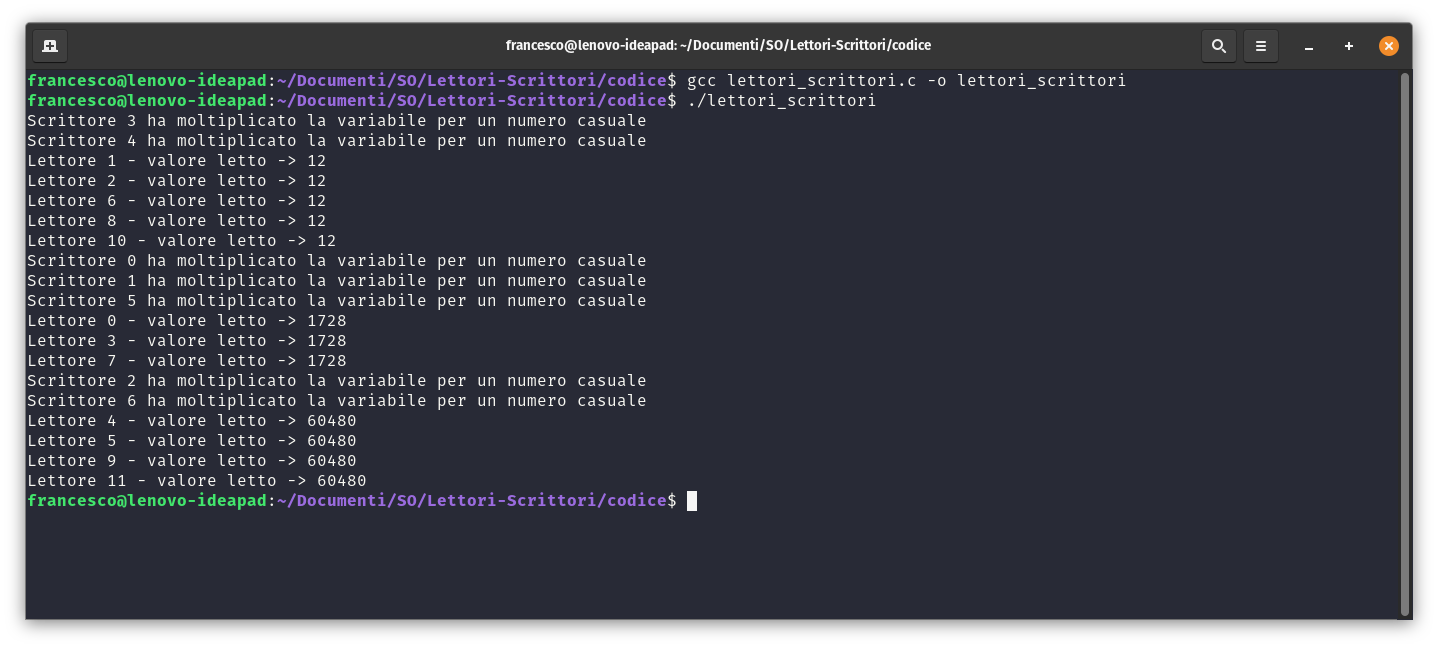
\includegraphics[width=1.03\linewidth]{img/esecuzione/programC1}
			\label{fig:programc1}
		\end{figure}
	\end{frame}
	\begin{frame}[fragile]
		\frametitle{Seconda esecuzione}
		\begin{figure}
			\centering
			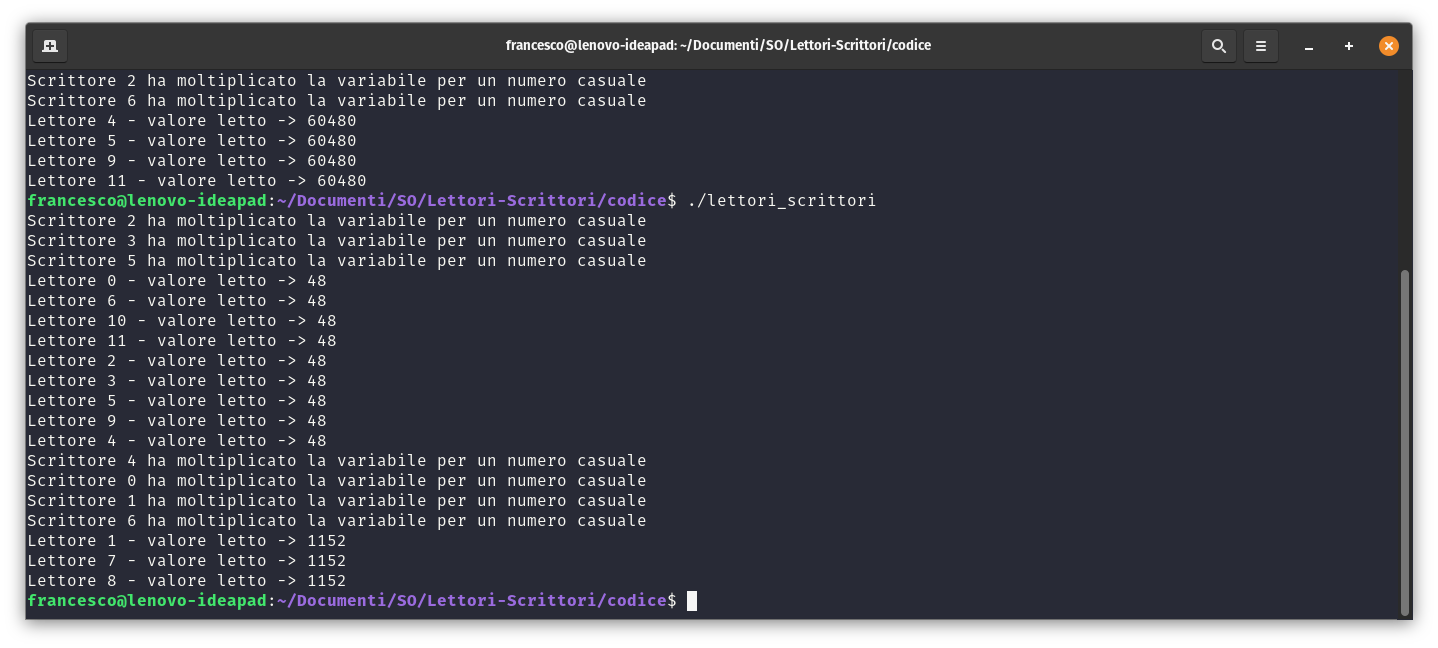
\includegraphics[width=1.03\linewidth]{img/esecuzione/programC2}
			\label{fig:programc1}
		\end{figure}
	\end{frame}

 %---Esecuzione Java----%
	\begin{frame}[fragile]
		\frametitle{Prima esecuzione}
		\begin{figure}
			\centering
			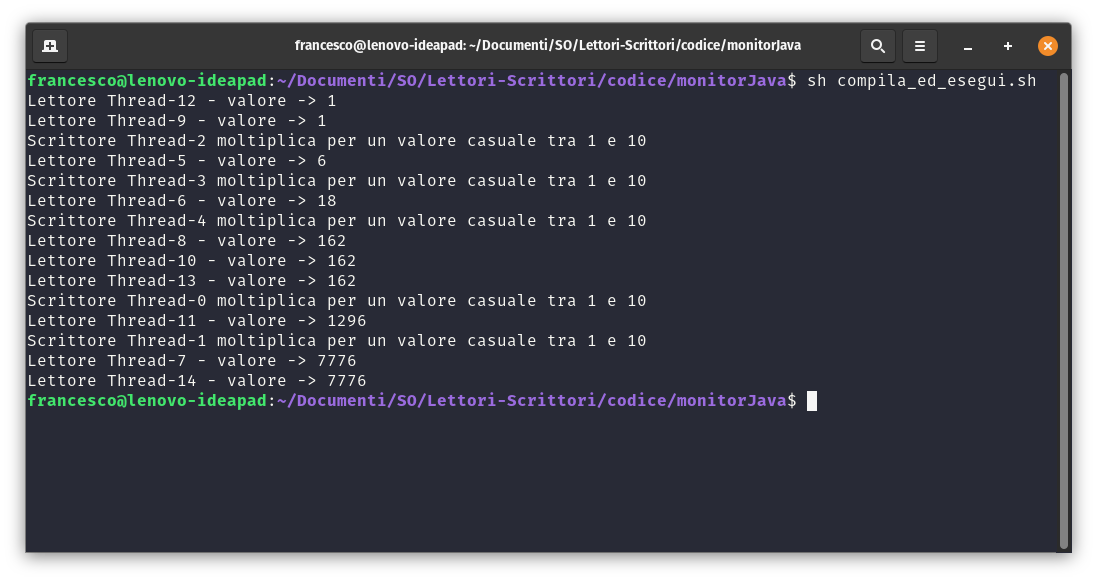
\includegraphics[width=1.03\linewidth]{img/esecuzione/programJ1}
			\label{fig:programc1}
		\end{figure}
	\end{frame}

	\begin{frame}[fragile]
		\frametitle{Seconda esecuzione}
		\begin{figure}
			\centering
			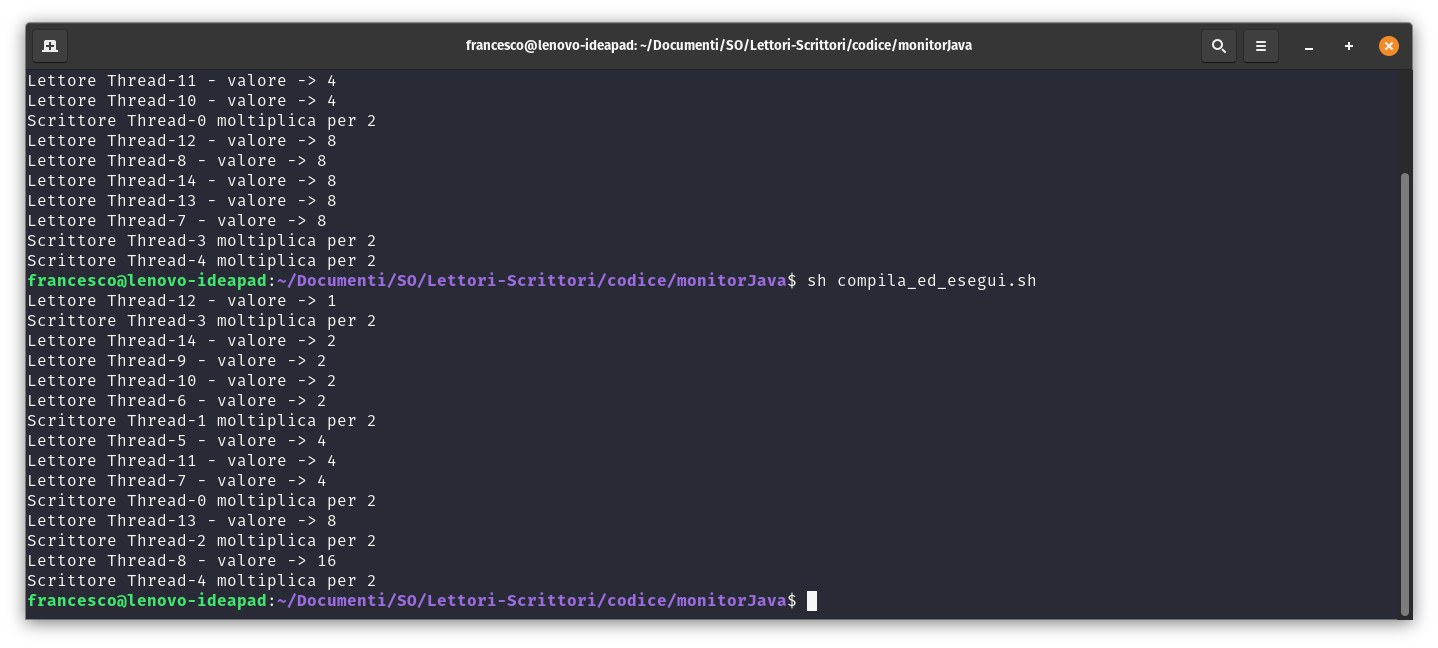
\includegraphics[width=1.03\linewidth]{img/esecuzione/programJ2}
			\label{fig:programc1}
		\end{figure}
	\end{frame}
	

	%------------------------------------------------
	
	%------------------------------------------------
	
	\begin{frame}
		\centerline{Link al repository con i sorgenti delle soluzioni viste e delle slides.}
		
		\centerline{\href{https://github.com/FrancescoLucia/Lettori-Scrittori.git}{https://github.com/FrancescoLucia/Lettori-Scrittori.git}}
	\end{frame}
	
	%----------------------------------------------------------------------------------------
	
\end{document} 